
\chapter{Gradient Fields}

This chapter covers the following ideas. 

% A list of objectives for the chapter
%\begin{enumerate}
%\item ...
%\end{enumerate}

\begin{enumerate}
\item Compute work done by a non-constant force $\vec F$ along a
  non-straight curve $C\colon\vec r(t)$.
\item Define and compute flow and circulation along a curve using the
  ideas from computing work.  Be able to compute flow along piecewise
  smooth curves. Give an application of flow in terms of fluid flow.
\item Compute the flux in the plane of a vector field $\vec F$ across
  a smooth curve $C\colon\vec r(t) = \langle x(t),y(t)\rangle$.  Give an
  application of flux in terms of fluid flow.
\item Be able to draw vector fields and determine if a given field is a
  gradient field (hence conservative)
\item Use the fundamental theorem of line integrals to greatly
  simplify work calculations.
\end{enumerate}

%%% Local Variables: 
%%% mode: latex
%%% TeX-master: "../multivariable-calculus"
%%% End: 
%$

\section{Work}

If a constant force $\vec F$ acts on an object through a displacement
in a straight line, then work is {$ W= \vec F\cdot \vec r $} (we use the
dot product).  If the displacement is not linear or the force is not
constant, then this formula breaks down. To find work done by a
non-constant force $\vec F$ along an arbitrary curve $\vec r$, start
by breaking the curve up into little pieces $\Delta \vec r = \vec T \Delta s$
(direction times magnitude, where $\vec T$ is the unit tangent
vector). On each little piece of the curve, the force is approximately
constant, and the displacement is approximately a straight line, so we
approximate the work done on each little piece as {$ \Delta W \approx \vec F \cdot \Delta
\vec r = \vec F \cdot \vec T \Delta s $}.  Sum the little pieces of work to get an
approximate total work {$ W \approx \sum \vec F \cdot \vec T \Delta s $}.  Taking limits
gives 
$$%\displaystyle
W = \int_C \vec F\cdot \vec T \,ds 
= \int_a^b\vec F\cdot \frac{\vec r'}{|\vec r'|}|\vec r'| dt 
= \int_a^b\vec F\cdot \vec r' dt 
= \int_C \vec F\cdot d\vec r.$$
(We use the differential notation {$ d\vec r= \vec r' dt $}, which
comes from the equation {$ \frac{d\vec r}{dt} = \vec r' $}.)
If {$ \vec F = \langle M,N,P\rangle $} for some functions $M,N$, and
$P$, then the work can be written 
$$W = \int_C \langle M,N,P\rangle\cdot\langle dx,dy,dz\rangle 
= \int_C Mdx+Ndy+Pdz.$$ These many formulas are different ways of
representing the exact same quantity.

\subsection{Flow (synonym for work) and Circulation (work on a closed
curve)}
Flow along a curve $C$ is a measure of how much fluid (with velocity
field {$ \vec F = \langle M,N,P\rangle $}) flows along a curve {$C\colon \vec r(t)$ , $a\leq
  t\leq b$,} per unit time. This quantity is particularly useful in the
study of fluid mechanics, for example, studying how air flow near a
wing provides lift for an airplane. The component of the velocity in
the direction of the curve is the scalar projection $|\proj_{\vec
  T}\vec F| = \vec F\cdot \vec T$.  For each little piece of curve $ds$,
the product $\vec F\cdot \vec T ds$ is approximately how much fluid will
flow along this portion of the curve.  Summing these small bits of
flow gives the total flow by the line integral {$\int_C \vec F\cdot \vec T
  \,ds = \int_C \vec F\cdot d\vec r = \int_C Mdx+Ndy+Pdz $}. If the curve is a
simple closed curve (meaning it is piecewise smooth, starts and ends
at the same point, and does not cross itself), then flow along $C$ is
called circulation around $C$.  We sometimes add a closed circle to
the integral to emphasize this, as in {$ \oint_C \vec F \cdot d\vec r $}. 

The only difference between work, flow, and circulation is how we
interpret the vector field.  The computations are the same.


% A vector field is said to be
% \textbf{conservative} if circulation along every closed loop is zero,
% or equivalently if work calculations are independent of the path,
% i.e., only depend on starting and ending points.


\begin{example}
\marginpartop{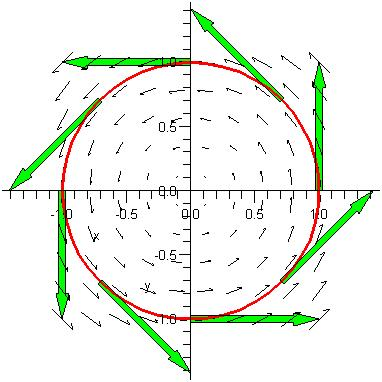
\includegraphics[width=\marginparwidth]{07-GradientFields/support/work-1}}%
Consider the vector field {$\vec F(x,y)=\langle-y,x\rangle$}.
The circulation of {$\vec F$} along a circle of radius $a$ that is
traversed counter-clockwise is found by first parametrizing the circle
$C\colon r(t) = \langle a\cos t,a\sin t\rangle$, $0\leq t\leq2\pi$ (so that we traverse it
counter-clockwise). Hence $\vec r'(t) = \langle-a\sin t,a\cos t\rangle$ and
$\int_C\vec F\cdot d\vec r = \int_0^{2\pi} \langle-y,x\rangle\cdot \langle-a\sin t,a\cos t\rangle dt =
\int_0^{2\pi} \langle-a\sin t,a\cos t\rangle\cdot \langle-a\sin t,a\cos t\rangle dt = \int_0^{2\pi}
a^2\sin^2 t+a^2\cos^2 t dt = \int_0^{2\pi} a^2 dt = 2\pi a^2$.  Notice that
the integral of a constant along an interval is always the length of
the interval multiplied by that constant.  This will speed up the
calculation of many integrals that we encounter throughout the
semester.
\end{example}

\begin{example}
\marginpartop{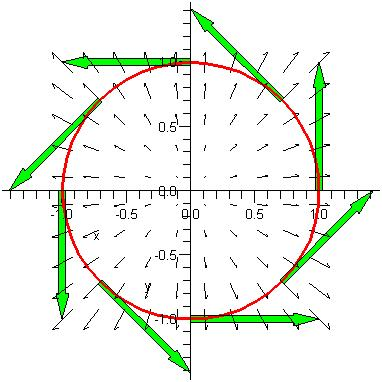
\includegraphics[width=\marginparwidth]{07-GradientFields/support/work-2}}%
Now consider the vector field {$\vec F(x,y)=\langle x,y\rangle$}.  To calculate
  the circulation of {$\vec F$} along a circle of radius $a$, we use
  the same parametrization as last time. This time using the formula
  $\int_C Mdx+Ndy$, we have $x=a\cos t$, $y=a\sin t$, $dx=-a\sin t$,
  $dy=a\cos t$, $M=x=a\cos t$, and $N=y=a\sin t$, so $\int_C Mdx+Ndy =
  \int_0^{2\pi} a\cos t (-a\sin t) + a \sin t (a\cos t) dt = \int_0^{2\pi} 0 dt
  = 0$.  Notice that the vector field is always orthogonal to the unit
  tangent vector, which is why the flow along $C$ is zero.
\end{example}

\begin{example}
\marginpartop{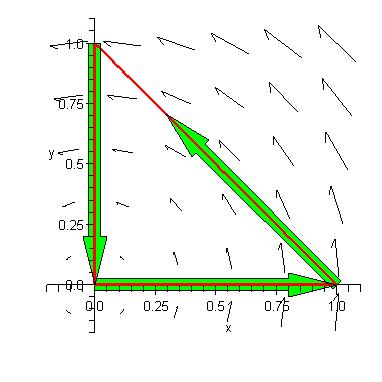
\includegraphics[width=\marginparwidth]{07-GradientFields/support/work-3}}%
Now consider the vector field {$\vec
  F(x,y)=\langle-y,x\rangle$} and the curve which forms the boundary of the
triangle with vertices $(0,0), (1,0), (0,1)$ and goes around
counter-clockwise. To find the work done by $\vec F$ through the
displacement along $C$ counter-clockwise (or the flow along $C$, or the circulation
around $C$), we first have to parametrize the curve.  This is a
piecewise smooth curve and, as such, is parametrized using 3 different
curves.  From (0,0) to (1,0), we get a direction vector for the line
segment by subtracting the points: $\langle1-0,0-0\rangle$. We then write
$C_1\colon\vec r_1(t) = \langle1,0\rangle t+\langle0,0\rangle$ for $0\leq t \leq 1$ (we know to stop at
1, because $\vec r_1(1)=\langle1,0\rangle$).  Similarly for the segment from (1,0)
to (0,1), we write $C_2\colon\vec r_2(t) = \langle-1,1\rangle t+\langle1,0\rangle$ for $0\leq t \leq
1$. For the segment from (0,1) to (0,0), we write $C_3\colon\vec r_3(t) =
\langle0,-1\rangle t+\langle0,1\rangle$ for $0\leq t \leq 1$. We then compute
$$\begin{array}{rlll}
  \oint_C \vec F\cdot d\vec r 
  &= \int_{C_1} \vec F\cdot d\vec r_1 &+ \int_{C_2} \vec F\cdot d\vec r_2 &+ \int_{C_3}
  \vec F\cdot d\vec r_3\\
  &= \int_0^1 \langle-y,x\rangle\cdot \langle1,0\rangle dt &+ \int_0^1
  \langle-y,x\rangle\cdot \langle-1,1\rangle dt &+ \int_0^1 \langle-y,x\rangle\cdot
  \langle0,-1\rangle dt\\
  &= \int_0^1 \langle-(0),(t+0)\rangle\cdot \langle1,0\rangle dt &+ \int_0^1
  \langle-(t+0),(1-t)\rangle\cdot \langle-1,1\rangle dt &+ \int_0^1
  \langle-(1-t),0\rangle\cdot \langle0,-1\rangle dt\\
  &= \int_0^1 0 dt &+ \int_0^1 (t+0)+(1-t)dt &+ \int_0^1 0 dt\\
  &= 0 &+ 1 &+ 0 \\
  &= 1.
\end{array}$$
\end{example}

\section{Flux across a smooth curve} 

Any simple closed curve (piecewise smooth, doesn't cross itself, and
starts and ends at the same point) divides the plane into two regions,
which we will call the inside and outside of the curve. Just as flow
measures the rate at which fluid moves \emph{along} a curve, flux
measures the rate at which fluid moves \emph{across} a simple closed
curve.  By convention, if fluid is flowing out of the region, then there
is a positive flux across the curve which is the boundary of the
region. If you were to turn on a faucet at the origin and let water
flow onto the plane, the water would flow outwards, and the flux would
be positive across any curve which encircled the origin.
Alternatively, if you placed the drain of a sink at the origin, then
flux across a curve encircling the origin would be negative (i.e.,
water would be flowing into the region bounded by the curve).

In order to determine the flux across a curve, we need a vector
pointing out of the curve.  Let $\vec n$ be an outward-pointing unit
normal vector.  Then $\vec F\cdot \vec n$ is the component of $\vec F$ in
the outward normal direction. Break up the curve into small bits of
curve $ds$.  Then $d\text{Flux} = \vec F\cdot \vec n \,ds$ is the small
amount of fluid which flows across each small bit $ds$ of
curve. \textbf{For the following formula, we will assume that we are
  traversing the curve counter-clockwise.}  If {$\langle dx,dy\rangle$} represents
the tangential direction in the counter-clockwise direction, then {$\langle
  dy,-dx\rangle$} gives the direction of the outward-pointing normal (we can
see this since the dot product with the tangential vector is zero, and
the vector points outward). A unit outward normal vector is hence $
\frac{\langle dy,-dx\rangle}{\sqrt{dy^2+dx^2}}$. For flux across a curve $C$, we
add up the small bits of flux to get the formula 

\begin{align*}
  \text{Flux } &= \int_C\,d\text{Flux} = \int_C\vec F\cdot \vec n \,ds = \int_C\vec
  F\cdot \frac{\langle dy,-dx\rangle}{\sqrt{dy^2+dx^2}} \sqrt{dx^2+dy^2} 
  = \int_C \langle M,N\rangle
  \cdot <dy,-dx> \\&= \int_C Mdy-Ndx.
\end{align*}
  In order to use this last formula, we
\emph{must} be traversing the curve in a counter-clockwise direction
(otherwise, $\langle dy,-dx\rangle$ won't be an outward-pointing normal vector).

\begin{example}
\marginpartop{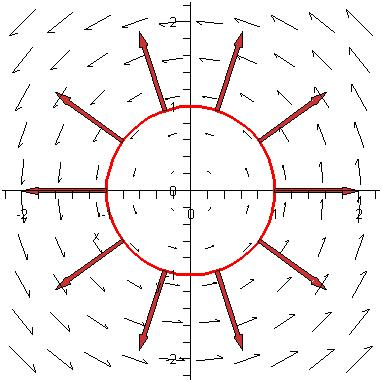
\includegraphics[width=\marginparwidth]{07-GradientFields/support/flux-1}}%
 Consider the vector field {$\vec F(x,y)=\langle-y,x\rangle$}.  The flux of
  {$\vec F$} across a circle of radius $a$ is found by first
  parametrizing the circle $C\colon r(t) = \langle a\cos t,a\sin t\rangle$.  Hence $\vec
  r'(t) = \langle-a\sin t,a\cos t\rangle$, or $dx=-a\sin t$ and $dy = a\cos
  t$. Hence we have $\int_C Mdy-Ndx = \int_0^{2\pi} (-a\sin t)(a\cos t)-(a\cos
  t)(-a\sin t)dt = \int_0^{2\pi} 0 dt = 0$.  In other words, no fluid is
  moving across the curve, in or out of the region.  Notice that this
  spin vector field is always orthogonal to the outward normal. This should
  visually show that the flux is zero. It is valuable to look at a
  picture and try to decide if the flux is zero, positive, or
  negative, as this will give you some intuition about flux.
\end{example}

\begin{example}
\marginpartop{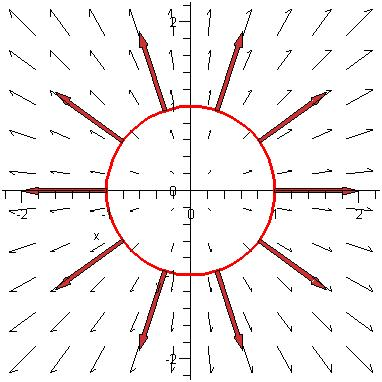
\includegraphics[width=\marginparwidth]{07-GradientFields/support/flux-2}}%
 Consider the vector field {$\vec F(x,y)=\langle x,y\rangle$}.  We use the same
  parametrization as the previous examples, so $x=a\cos t$, $y=a\sin t$,
  $dx=-a\sin t$, $dy=a\cos t$, $M=x=a\cos t$, and $N=y=a\sin t$. This gives the
  flux of $\vec F$ across $C$ as $\int_C Mdy-Ndx = \int_0^{2\pi} a\cos t
  (a\cos t) - a \sin t (-a\sin t) dt = \int_0^{2\pi} a^2(\cos^2t+\sin^2t)
  dt = 2\pi a^2$.  If our vector field is giving the velocity of water
  in meters per second, then this result says that $2\pi a^2$ square
  meters of water is flowing out of the circle per second.  You should
  notice that the vector field in this instance is always pointing out
  of the circle. Since the vector field and the outward normal are in
  the same direction, the flux is positive. Fluid is moving out of the
  interior of the circle.
\end{example}

\begin{example}
\marginpartop{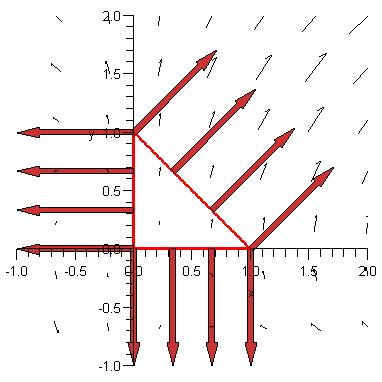
\includegraphics[width=\marginparwidth]{07-GradientFields/support/flux-3}}%
 Consider the vector field {$\vec F(x,y)=\langle xy,x+y\rangle$} and the curve $C$
  which forms the boundary of the triangle with vertices $(0,0),
  (1,0), (0,1)$. We first parametrize $C$ by finding a parametrization
  for each curve (remember: we need to traverse in a counter-clockwise
  direction to use our formula). This already done above, and we had
  the three curves $C_1\colon\vec r_1(t) = \langle1,0\rangle t+\langle0,0\rangle$ for $0\leq t \leq 1$,
  $C_2\colon\vec r_2(t) = \langle-1,1\rangle t+\langle1,0\rangle$ for $0\leq t \leq 1$, and $C_3\colon\vec
  r_3(t) = \langle0,-1\rangle t+\langle0,1\rangle$ for $0\leq t \leq 1$. We then compute the flux of
  $\vec F$ across $C$ as $$\begin{array}{rlll} \oint_C Mdy-Ndx &= \int_{C_1}
    (M)(0) - (x+y)(1)dt &+ \int_{C_2} (xy)(1)-(x+y)(-1)dt &+
    \int_{C_3} (xy)(-1)-(N)(0)dt\\
    &= \int_0^1 - (t+0) dt &+ \int_0^1 (1-t)(t)+(1-t)+(t) dt &+ \int_0^1
    (0)(1-t)(-1) dt\\
    &= \int_0^1 - t dt &+ \int_0^1 t-t^2 + 1  dt &+ \int_0^1 0 dt\\
    &= -\frac{1}{2} &+ \frac{1}{2}-\frac{1}{3}+1 &+ 0 \\
    &= \frac{2}{3}
  \end{array}$$
\end{example}


\section{Gradients, Potentials, and the Fundamental Theorem}

When the output dimension of a function is one, {i.e.,
  $f\colon{\mathbb{R}}^n\to {\mathbb{R}}^1$}, then the derivative is called
the gradient and is written in vector form as {$\nabla f = \langle f_x,f_y,f_z\rangle$}.
If a vector field {$\vec F = \langle M,N,P\rangle$} is the gradient of some
function {$f$} (so that {$\nabla f= \vec F$}), then we say that the vector
field {$\vec F$} is a gradient field, and the function {$f$} is called
a potential for {$\vec F$}. The potential of a gradient field appears
in differential equations, engineering, physics, and probably many
other places.

\subsection{Test for a gradient field}

If a vector field $\vec F$ is a gradient field (meaning there is an
$f$ such that $\nabla f=\vec F$), and the potential $f$ has continuous
second derivatives, then the second-order mixed partial derivatives
must be equal, namely $f_{xy}=f_{yx}$, $f_{xz}=f_{zx}$, and
$f_{yz}=f_{zy}$. So if $\vec F = \langle M,N,P\rangle$ is a gradient field and the
components of $\vec F$ have continous partial derivatives, then since
$M=f_x$, $N=f_y$, and $P=f_z$, we must have $M_y=N_x$, $M_z=P_x$, and
$N_z=P_y$. If these partial derivatives do not agree, then the vector
field cannot be a gradient field.  This gives us an easy way to
determine that a vector field is \emph{not} a gradient field.

\begin{example}
The vector field $\langle-y,x,-yx\rangle$ is not a
  gradient field because {$M_y=-1$} is not equal to {$N_x=1$}.
\end{example}
To prove a vector field does not have a potential, you must show that
either $M_x\neq N_y$, $M_z\neq P_x$, or $N_z\neq P_y$. It is insufficient to
say ``There is no potential because I could not find one.''


When $\vec F$ is defined on a ``nice'' set (which is almost always
true in real life) and has continous partial derivatives, the check
works the other way as well.  For example, if a vector field $\vec
F=\langle M,N,P\rangle$ is defined on all of $\mathbb{R}^3$ (which is a ``nice''
set), $\vec F$ has continous partial derivatives, and $M_y=N_x$,
$M_z=P_x$, and $N_z=P_y$, then $\vec F$ is a gradient field (i.e.,
there is a potential function $f$ such that $\vec F = \nabla f$).  This
gives us a very nice way of checking if a vector field is a gradient
field.  See Section~\ref{sec:nice-sets} for a discussion of what a ``nice'' set is
and what happens when a vector field is not defined over a ``nice''
set.


\begin{example}
The vector field $\vec F=\langle x,z,y\rangle$ is
  a gradient field because $\vec F$ is defined on all of
  $\mathbb{R}^3$, each component has continous partial derivatives,
  and $M_y=0=N_x$, $M_z=0=P_x$, and $N_z=1=P_y$.  Notice that
  $f=x^2/2+yz$ gives $\nabla f = \langle x,z,y\rangle=\vec F$.
\end{example}

\textbf{Exact differential forms:} A \emph{differential form} is an
expression of the form {$Mdx+Ndy+Pdz$}.  On the other hand, if we have
a function $f(x,y,z)$, the differential of $f$ is 
$$df = Df d\vec x
= \begin{bmatrix}f_x&f_y&f_z
\end{bmatrix}\begin{bmatrix}dx\\dy\\dz\end{bmatrix}=f_x dx+f_y dy+f_z
dz.$$ If a differential form is actually the differential of a
function {$f$}, then the differential form is said to be
\textbf{exact}.  The function {$f$} is called a potential for the
differential form.  Notice that {$Mdx+Ndy+Pdz$} is exact if and only
if {$\vec F = \langle M,N,P\rangle$} is a gradient field.

\begin{example}
The differential form $-ydx+xdy-yxdz$ is not
  exact since the field $\langle-y,x,-yx\rangle$ is not a gradient
  field (see above).  The differential form $xdx+zdy+ydz$ is exact
  since the field $\langle x,z,y\rangle$ is a gradient field (see
  above).
\end{example}
\subsection{Finding a potential (undoing a total derivative):} If we know
$\vec F=\langle M,N,P\rangle$ is a gradient field, then to find a potential
function $f$, we simultaneously solve the differential equations
$f_x=M$, $f_y=N$, and $f_z=P$.  In other words, we have to find a
function $f$ which is a solution of all three integrals $\int Mdx$, $\int
Ndy$, and $\int Pdz$.  Essentially, this is undoing the total
derivative. The following examples illustrate two methods of doing so.
The first method matches the book, while the second is quicker route which
simplifies the general idea.

\textbf{Method 1:} Consider the vector field $\vec
F=\langle2xy+x,x^2-3z,-3y+z^2\rangle$. Since $D\vec F$ is continuous and
$M_y=2x=N_x$, $M_z=0=P_x$, and $N_z=-3=P_y$, the vector field $\vec F$ is a
gradient field, so $\vec F$ has a potential function $f$, and $f_x=M$, $f_y=N$, and $f_z=P$.
\begin{enumerate}
\item Integrate $\int f_x\,dx=\int M\,dx$ to get $\int 2xy+x\,dx =
  x^2y+x^2/2+A(y,z)=f$, where $A$ is a constant with respect to $x$,
  which means that $A$ may actually be a function of $y$ and $z$.
\item Differentiate $f$ with respect to $y$ to obtain
  $N=f_y=\frac{\partial}{\partial y}[x^2y+x^2/2+A(y,z)] = x^2+A_y(y,z)$. Therefore,
  $x^2-3z=x^2+A_y(y,z)$, so $A_y(y,z)= -3z$ and $f_y=x^2-3z$.
\item Integrate $A_y$ with respect to $y$ to obtain $A(y,z)=\int -3z dy =
  -3yz+B(z)$, where $B$ is a constant with respect to $y$, which means
  that $B$ may actually be a function of $z$.  Thus,
  $f=x^2y+x^2/2-3yz+B(z)$.
\item Differentiate $f$ with respect to $z$ to get $P=f_z=-3y+B_z(z)$,
  so $-3y+z^2=-3y+B_z(z)$, so $B_z(z)=z^2$.
\item Integrate $B$ with respect to $z$ to get $B(z)=\int z^2 dz =
  z^3/3+C$ for some constant $C$ (and this is really a numeric
  constant!).  Hence a potential is $f= x^2y+x^2/2-3yz+z^3/3+C$ for
  any constant $C$.
\end{enumerate}

It is easy to check that $f$ is a potential by computing $\nabla f =
\langle2xy+x,x^2-3z,-3y+z^2\rangle$, which should equal $\vec F$.
Please, \emph{please} always check your answer by calculating $\nabla
f$ and making sure that it equals $\vec F$.

\textbf{Method 2:} As an alternative approach, integrate all three
functions simultaneously, ignoring the constants, to get $\int M dx =
x^2y+x^2/2$, $\int N dy = x^2y+-3yz$, and $\int P dz = -3yz +z^3/3$.
Provided a potential exists, then the function $f$ is formed by
summing these integrals, ignoring duplicated terms. Since $x^2y$ and
$-3yz$ appear in multiple integrals (are duplicated terms), we include
them once in the sum to obtain $f= x^2y+x^2/2-3yz+z^3/3$ as a
potential function. This method will work if a potential exists.

\begin{example}
  \textbf{Method 2 - second example:} As another example, consider the
  vector field $\vec F(x,y,z) = \langle
  xy+yz+1,x^2/2+xz-3z,xy-3y\rangle$.  The test for a gradient field
  shows $M_y=x+z=N_x$, $M_z=y=P_x$, and $N_z=x-3=P_y$, which means
  that $\vec F$ is a gradient field.  A potential is found by
  integrating $\int xy+yz+1 dx = \frac12x^2y+xyz+x$, $\int x^2/2+xz-3z
  dy =\frac12x^2y+xyz-3yz$, and $\int xy-3y dz = xyz-3yz$. The term
  $xyz$ appears in all three results, $\frac12x^2y$ appears in the
  first two results, and $-3yz$ appears in the last two results. A
  potential is found by summing the terms (not repeating duplicates)
  to obtain $f(x,y,z) = \frac 1 2 x^2y+xyz+x-3yz$.  Again, please
  check the answer.
\end{example}
When using the second approach, any time a term contains more than one
variable, that term will appear in more than one integral. For the
vector field $\vec F = \langle yz,xz,yz\rangle$, the integral $\int Mdx = xyz$
contains $x,y,$ and $z$, so the integral with respect to $y$ and $z$
must also contain this term.  We compute $\int Ndy = xyz$ and $\int Pdz =
yz^2/2$, and notice that the same term appears in the $y$ integral,
but not in the $z$ integral. Because $\int Mdx = xyz$ contains all three
variables but does not appear as a term in the third integral, we
should be able to show using the test for a gradient vector
field that there is no potential.  Notice that $P_x=0$ and $M_z=y$
are not equal, which means that $\vec F$ is not a gradient field.


\subsection{The Fundamental Theorem of Line Integrals (why potentials
are useful)}
When a vector field is a gradient field, there is a simple way to
compute the work done by $\vec F$ along a curve $\vec r(t)$, $a\leq t\leq b$.
First, find a potential $f$ for $\vec F$, meaning $\vec F =\nabla f$. Let
$A=\vec r(a)$ be your starting point and $B=\vec r(b)$ be your ending
point. The work done is simply the difference in the potential from
$A$ to $B$.  In other words, 
$$W =\int dW= \int_a^b \vec F \cdot \vec r'(t) \,dt =f(B)-f(A).$$ 
This work depends only on the starting and ending points, not the path
chosen, so we say that the work done is independent of path.  The
reason for the word ``potential'' has to do precisely with the fact
that differences in potential convert ``potential energy'' to work
(another measure of energy).

\begin{example}
Suppose $\vec F = \langle x+y,x+y\rangle$ and $C$ is the upper
semicircular curve in the plane starting at $(1,0)$ and ending at
$(-1,0)$, followed by the straight line segment from $(-1,0)$ to
$(0,0)$. A potential for $\vec F$ is $f(x,y) =
\frac{1}{2}x^2+xy+\frac12 y^2$ (check this!).  The flow of $\vec F$
along $C$ is $\int_C \vec F \cdot d\vec r = f(0,0)-f(1,0) =-\frac{1}{2} $ by
the fundamental theorem of line integrals.  Without the fundamental
theorem of line integrals, we write $r_1(t) = \langle\cos t,\sin t\rangle$, $0\leq t\leq
\pi$, and $r_2(t) = \langle t,0\rangle$, $-1\leq t\leq 0$, and then compute $\int_C \vec F \cdot
d\vec r = \int_0^\pi \langle\cos t+\sin t,\cos t+\sin t\rangle\cdot\langle-\sin t, \cos t\rangle dt
+\int_{-1}^0\langle t+0,t+0\rangle\cdot\langle1,0\rangle dt = 0-\frac12$.
\end{example}


Note that since work and flow are calculated exactly the same way,
this also gives an easy way to calculate flow.  Also notice that if
$A=B$, then the work is zero.  This also says that the circulation
around any simple closed curve is zero in a gradient field.

\subsubsection{Conservative Vector Fields}

Many places (including our book), a gradient vector field is also
called a \textbf{conservative} vector field.  However, some other
people define a conservative vector field as a vector field in which
work is independent of path (this ``conservation of energy'' is what
leads to the term ``conservative field'').  For vector fields defined
on a ``nice'' set, like all of $\mathbb{R}^2$ or all of
$\mathbb{R}^3$, these properties are all equivalent.  In more esoteric
cases (that don't come up very often in practice), these properties
may not be equivalent.  See Section~\ref{sec:nice-sets} for a
discussion of what a ``nice'' set means and what happens when you have
a vector field defined on a set that is not so nice.


\subsubsection{Integrating over a region by evaluating on the
  boundary}

A motif\footnote{A motif is ``a dominant idea or central theme.''
  (Merriam-Webster Dictionary)} that
you will see in the major theorems that we will discuss is the idea
that we can integrate a function over a region by simply evaluating
a related function on the boundary of the region.  The fundamental
theorem of calculus essentially says this: if we want the integral of
$f'(x)$ over the region $[a,b]$, then we only have to evaluate $f$ on
the boundary of the region, the points $a$ and $b$.  The fundamental
theorem of line integrals has the same idea: to calculate the integral
of $\nabla f\cdot \vec r'(t)$ over a curve $C$, then it is only necessary to
evaluate $f$ on the boundary of the curve, the starting and ending
points.  This idea is rather powerful---no matter what happens in the
interior of the region (provided it stays sufficiently
nice), as long as the boundary stays the same, the integral will be
the same.

\subsection{The Fundamental Theorem of Line Integrals}

The remainder of this section deals with explaining exactly why the
fundamental theorem of line integrals works. Essentially, it is an
extension of the fundamental theorem of calculus. Since we will be
seeing this theorem again in several different ways throughout the
course, we will discuss it in some depth now.

\subsubsection{The Fundamental Theorem of Calculus}

Because the fundamental theorem of line integrals is basically an
extension of the fundamental theorem of calculus, the proofs are
closely related.  Let's review the ideas behind the fundamental
theorem of calculus.

You can think of the derivative of $f$ as a density which measures
change in $f$ per unit length (i.e., $f'$ is a ``change density''). We
write $\frac{dy}{dx}\approx \frac{\Delta y}{\Delta x} = \frac{f(x+h)-f(x)}{(x+h)-x}$.

The Fundamental Theorem of Calculus, $f(b)-f(a)=\int_a^b f' dx$, says
that you can find the total change in a function $f(b)-f(a)$ by adding
up little changes $dy=f'dx$ (i.e., ``change density'' times length of
a small piece of the interval) over small segments of the interval
$[a,b]$.  Begin by breaking the interval {$[a,b]$} up into little
pieces {$a=x_0<x_1<x_2<\cdots <x_{n-1}<x_n=b $} so that the $i$th interval
has width $\Delta x_i = x_i-x_{i-1}$. The total change {$f(b)-f(a)$} in $f$
is approximated by adding up little changes $\Delta
y_i=f(x_i)-f(x_{i-1})$. If we multiply and divide by $\Delta x_i$, then
each little change is $\Delta y_i=\frac{f(x_i)-f(x_{i-1})}{\Delta x_i}\Delta x_i =
\frac{\Delta y_i}{\Delta x_i}\Delta x_i \approx \frac{dy}{dx}\Delta x_i$, which is approximately
the density $\frac{dy}{dx}$ times a length $dx$. The mean value
theorem is the theoretical tool which allows us to remove the
approximately equal and write $\frac{\Delta y_i}{\Delta x_i}\Delta x_i =
\frac{dy}{dx}(c_i)\Delta x_i$ for some $c_i$ between $x_{i-1}$ and $x_i$.
Summing the approximate changes and taking a limit as $\Delta x_i\to 0$ gives
the fundamental theorem of calculus. Notationally, this is all
summarized as
\begin{align*}
f(b)-f(a) 
&= f(b)-f(x_{n-1}) + f(x_{n-1})-f(x_{n-2})+\cdots + f(x_{2})-f(x_{1})+
f(x_{1})-f(x_{a}) \\
&= \sum f(x_i) - f(x_{i-1}) 
= \sum\frac{f(x_i) - f(x_{i-1})}{ \Delta x_i}\Delta x_i  
= \sum\left(\frac{\Delta y_i}{ \Delta x_i}\right)\Delta x_i  
\approx \sum\frac{dy}{ dx}\Delta x_i 
\end{align*}
Taking limits gives us {$ f(b)-f(a) = \int_a^b f'(x)dx $}, the
fundamental theorem of calculus. 

\subsubsection{The Fundamental Theorem of Line Integrals}
Let {$ f(x,y,z) $} be a function. Let $C$ be a smooth space curve,
parametrized by {$ \vec r(t)$, $a\leq t\leq b $}. Let {$ A=\vec r(a) $} and {$
B=\vec r(b) $} be the starting and ending points of the curve. The total
change in {$ f $} from {$ A $} to {$ B $} is $f(B)-f(A) = f(\vec
r(b))-f(\vec r(a))$.  The fundamental theorem of line integrals states
that 
$$ f(B)-f(A) = \int_C d(f\circ \vec r) = \int_C \nabla f\cdot d\vec r = \int_a^b \nabla f \cdot \vec
r' dt. $$ 

The change density is the change in $f$ (i.e., $df$) per unit length
$ds$ (we use arc length for length because motion is along a
curve). The change density can be written $\frac{d f}{d s} = \frac
{df}{dt} \frac{dt}{ds}=\frac {df}{dt} \frac{1}{ds/dt}=\frac{d(f\circ \vec
  r)}{dt}\frac{1}{ds/dt}$ (remember $\frac {dt}{ds}=\frac{1}{ds/dt}$
by the inverse function theorem). The chain rule gives
$\frac{df}{dt}\frac 1 {ds/dt} = Df D\vec r \frac{1}{ds/dt} = \nabla f \cdot
\vec r' \frac{1}{ds/dt}$. Multiplication by $ds/dt$ gives
$\frac{df}{dt} = \nabla f \cdot \vec r'$, or in differential notation, $df = \nabla
f \cdot \vec r' dt$.

As before, begin by breaking the interval $[a,b]$ up into little
pieces {$ a=t_0<t_1<t_2<\cdots <t_{n-1}<t_n=b $}.  Total change in $f$ is
then
\begin{align*}
f(B)-f(A) 
&= f(\vec r(b))-f(\vec r(t_{n-1})) + f(\vec r(t_{n-1}))-f(\vec
r(t_{n-2})) +\cdots + f(\vec r(t_{1}))-f(\vec r(t_{a})) \\
&= \sum f(\vec r(t_i)) - f(\vec r(t_{i-1})) 
= \sum\Delta (f\circ\vec r) \\
&= \sum\frac{\Delta(f\circ \vec r)}{ \Delta t_i}\Delta t_i  
= \sum (D(f\circ \vec r)(c_i)) \Delta t_i 
= \sum DfD\vec r \Delta t_i 
= \sum \nabla f\cdot \vec r' \Delta t_i, 
\end{align*}
where the $c_i$ points are again given by the mean value theorem.  Taking
limits gives us the fundamental theorem of line integrals: $
f(B)-f(A)= \int_C \nabla f\cdot \vec r'dt = \int_C\nabla f\cdot d\vec r $.

\subsection{``Nice'' sets}
\label{sec:nice-sets}

Here we will discuss in (brief) technical detail what a ``nice'' set
is and what goes wrong when you have a set that is not so nice.  This
would all be explored in much more detail in an advanced calculus, real
analysis, or algebraic topology class.

Let $\vec F=\langle M,N,P\rangle$ be continuous on an open set $D$.  In the
following chart, the arrows represent implications (i.e., if there is
an arrow from one statement pointing to another, then the first
statement being true implies that the second statement is true).  A
label on the arrow means that the condition has to be satisfied for
the implication to be hold.  The definitions of the terms are in the
book (or you can ask me). 

\begin{figure}[h]
  \centering
 \begin{tikzpicture}[description/.style={fill=white,inner sep=2pt}]
    \matrix (m) [matrix of math nodes, row sep=8em,
    column sep=16em, text height=1.5ex, text depth=0.25ex]
    { F=\nabla f & \displaystyle\int_C\vec F\cdot d\vec r \text{ is independent of path} \\
     M_y=N_x, M_z=P_x, N_z=P_y  & \displaystyle\oint_C \vec F\cdot d\vec r=0 \text{ (closed path $C$)}\\ };
    \path[>=latex,->,line width=1pt]
    (m-1-1.north east) edge [bend left=5] (m-1-2.north west)
    (m-1-1) edge  node[auto] {$\vec F$ has continous partials} (m-2-1)
    (m-1-2) edge [bend left=5] node[auto] {$D$ connected} (m-1-1)
    (m-1-2) edge [bend left=10] (m-2-2)
    (m-2-1) edge node[above] {$\vec F$ has continous partials} node[below] { $D$ connected and simply connected} (m-2-2)
    (m-2-2) edge [bend left=10] (m-1-2);
    
\end{tikzpicture}
  
  \caption{Equivalences for nice sets}
  \label{fig:equivalences}
\end{figure}


Using terms from the book, a ``nice'' set is a set that is open,
connected, and simply connected.  Roughly, this means that $D$ does
not include its boundary and is a single region without any holes going
through it.  For such a ``nice'' set, all four statements in
Figure~\ref{fig:equivalences} are equivalent (i.e., either they are
all true or they are all false for a given vector field $\vec F$).

If the set $D$ is not connected, then path-independence does not imply
the vector field is a gradient field.  In this case, discrepancies can
occur between the two definitions for ``conservative vector field''.

There is a homework problem that shows that the bottom arrow
does not hold when $D$ is not simply connected.  When $D$ is not
connected and simply  connected, we lose the nice, easy test in the
lower left of the figure for determining exactly when a vector field
is a gradient field.







%%% Local Variables: 
%%% mode: latex
%%% TeX-master: "../multivariable-calculus"
%%% End: 





